\documentclass[a4paper, 12pt]{article}%тип документа

%%%Библиотеки
	%\usepackage[warn]{mathtext}	
	\usepackage[T2A]{fontenc} % кодировка
	\usepackage[utf8]{inputenc} % кодировка исходного текста
	\usepackage[english,russian]{babel} % локализация и переносы
	\usepackage{caption}
	\usepackage{listings}
	\usepackage{amsmath,amsfonts,amssymb,amsthm,mathtools}
	\usepackage{wasysym}
	\usepackage{graphicx}%Вставка картинок правильная
	\usepackage{float}%"Плавающие" картинки
	\usepackage{wrapfig}%Обтекание фигур (таблиц, картинок и прочего)
	\usepackage{fancyhdr} %загрузим пакет
	\usepackage{lscape}
	\usepackage{xcolor}
	\usepackage[normalem]{ulem}
	\usepackage{hyperref}

%%%Конец библиотек




%%%Настройка ссылок
	\hypersetup
	{
		colorlinks=true,
		linkcolor=blue,
		filecolor=magenta,
		urlcolor=blue
	}
%%%Конец настройки ссылок


%%%Настройка колонтитулы
	\pagestyle{fancy}
	\fancyhead{}
	\fancyhead[L]{Лабораторная работа}
	\fancyhead[R]{Талашкевич Даниил, группа Б01-009}
	\fancyfoot[C]{\thepage}
%%%конец настройки колонтитулы



							\begin{document}
						%%%%Начало документа%%%%


%%%Начало титульника
\begin{titlepage}

	\newpage
	\begin{center}
		\normalsize Московский физико-технический институт \\(госудраственный 			университет)
	\end{center}

	\vspace{6em}

	\begin{center}
		\Large Лабораторная работа по электричеству\\
	\end{center}

	\vspace{1em}

	\begin{center}
		\large \textbf{Влияние магнитного поля на проводимость полупроводников [3.3.6]}
	\end{center}

	\vspace{2em}

	\begin{center}
		\large Талашкевич Даниил Александрович\\
		Группа Б01-009
	\end{center}

	\vspace{\fill}

	\begin{center}
	Долгопрудный \\2021
	\end{center}
	
\end{titlepage}
%%%Конец Титульника



%%%Настройка оглавления и нумерации страниц
	\thispagestyle{empty}
	\newpage
	\tableofcontents
	\newpage
	\setcounter{page}{1}
%%%Настройка оглавления и нумерации страниц


					%%%%%%Начало работы с текстом%%%%%%
					
\textbf{Цель работы:} измерение зависимости сопротивления полупроводниковых образцов различной формы от индукции магнитного поля. \\

\textbf{Используемое оборудование:} электромагнит, милливеберметр или миллитесламетр (на основе датчика Холла), вольтметр, амперметр, миллиамперметр, реостат, образцы монокристаллического антимонида индия (InSb) $n$-типа.
                    
\section{Теоретическое введение}

В работе исследуется эффект зависимости электрического сопротивления от магнитного поля на примере диска Корбино (см. рис.).

\begin{figure}[h]
    \centering
    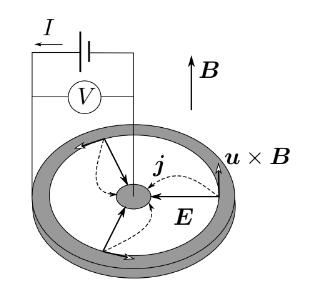
\includegraphics[width = 5 cm]{images/1.png}
    \caption{Диск Корбино}
    \label{karb}
\end{figure}

При отстутствии магнитного поля, направленного перпендикулярно плоскости диска, по диску течёт ток, определяемый по закону 

\begin{equation}
    I = \frac{U}{R_0}, \; R_0 = \frac{\ln{\frac{r_2}{r_1}}}{\sigma_0 2 \pi r h}
\end{equation}

Однако при включении магнитного поля индукции $B$ на частицы-переносчики тока начинает действовать сила Лоренца, из-за чего траектория частиц увеличивается в расстоянии, проходимом между двумя точками с фиксированной разницей потенциалов $U$.

В этом случае проводимость  равна 

\begin{equation}
    \sigma_r = \frac{\sigma_0}{1 + (\mu B)^2}
\end{equation}

Закон Ома преобразовывается в следующий вид:

\begin{equation}
    I = \frac{U}{R}, \; R = R_0 (1 + (\mu B)^2)
\end{equation}

Таким образом, зависимость $I(U)$ поменялась из-за геометрических особенностей диска Корбино. Такой эффект называют геометрическим магнетосопротивлением. В этой работе будут исследоваться зависимость сопротивления диска от магнитного поля, проверяться выше записанные формулы и исследоваться как влияет характер зависимости геометрических форм на зависимость $R(B)$.

\section{Экспериментальная установка}

Для исследование зависимости $R(B)$ используется следующая методика:

\begin{enumerate}
    \item Используется калибровка электромагнита (источника магнитного поля): находится зависимость индукции создаваемого магнитного поля от тока в контуре электродвигателя $B(I_m)$ (или $I_m(B)$), который регистрируется амперметром $A_1$, чтобы в дальнейшем считать величину магнитного поля с помощью тока в контуре $I_m$.
    \item При постоянной силе тока $I_0$, которая настривается с помощью сопротивления реостата в контуре с источником питания, меняется величина индукции магнитного поля, тем самым меняется напряжение $U$, подаваемое на диск Корбино. Исследуется зависимость $R(B)$ через калибровочную кривую и зависимость $U(I_m)$.
    \item Проводится тот же самый опыт с прямоугольной пластинкой с исследованием зависимости её сопротивления $R(B)$.
\end{enumerate}

\begin{figure}[h!]
    \centering
    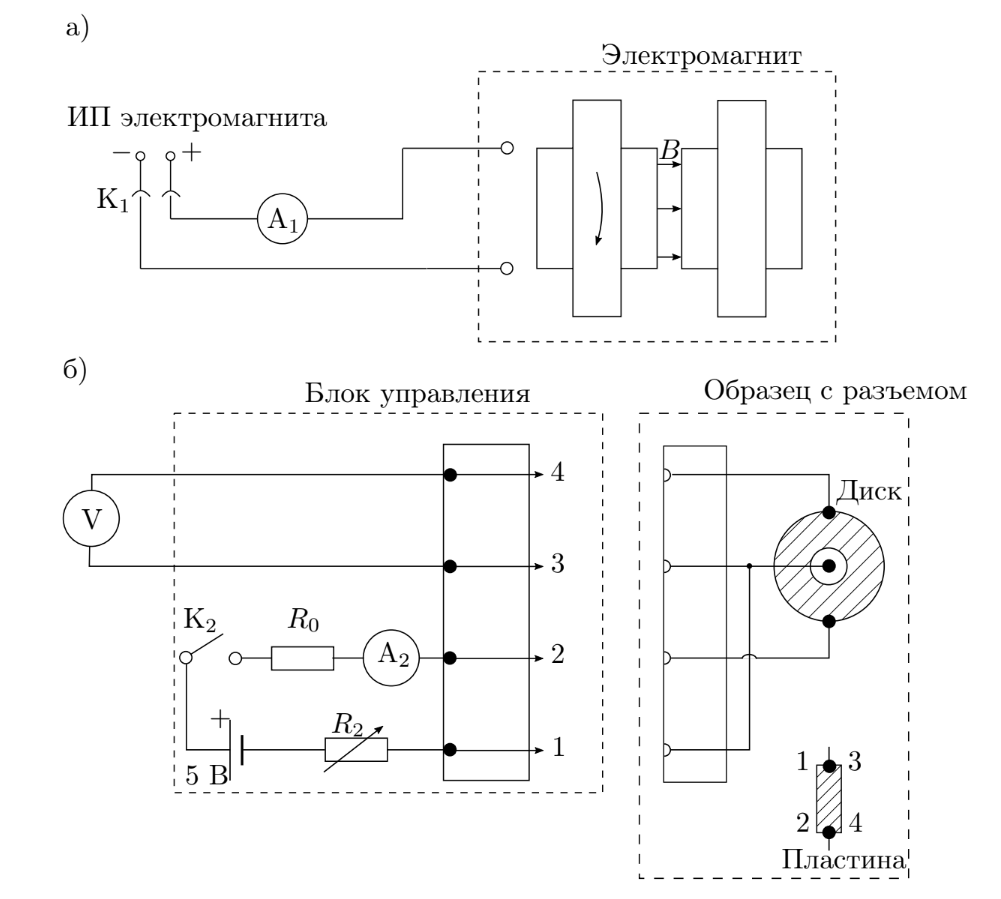
\includegraphics[width = 13 cm]{images/2.png}
    \caption{Схемы экспериментальных установок}
    \label{scheme}
\end{figure}


\section{Ход работы}

\subsection{Подготовка приборов к работе}

Включим вольтметр кнопкой "Сеть"

Присоединим диск Корбино через разъём к цепи питания. Убедившись, что реостат $R_{2}$ выведен на минимум тока, включим в сеть блок управления и тумблером $\mathrm{K}$ подключим образец.

Теперь определим диапазон изменения силы тока через образец. Для этого снова уберем ток до нуля и временно отключим образец от цепи. 

Установим все ручки регулировки источника питания магнита (GPR-11H30D) на минимум сигнала и включим источник в сеть. Установим обе ручки регулировки тока на максимум.

Используя ручки регулировки напряжения $R_{1}$ (сначала $fine$, затем $coarse$), определим диапазон изменения силы тока через электромагнит, чтобы выбрать, каким шагом следует увеличивать ток при калибровке магнита. 

Получили следующий диапазон изменения силы тока через электромагнит $0,05 - 0,40$ А.


\subsection{Калибровка электромагнита}

Сперва ознакомимся с устройством и принципом работы измерителя магнитной индукции Ш1-10.

Теперь при помощью прибора Ш1-10 исследуем зависимость индукции $B$ магнитного поля в зазоре от тока $I_{M}$ через обмотки магнита.

Проведем измерения магнитной индукции для 8 значений тока $I_{\mathrm{M}}$ через электромагнит. Так же убидились, что в отсутствие тока через магнит индукция $B$ практически равна нулю.


\begin{table}[!h]
\begin{center}
\begin{tabular}{|c|c|}
\hline I, A & B , мТс	\\
\hline $0,05$ & $71,4$ 	\\
\hline $0,10$ & $125,7$ 	\\
\hline $0,15$ & $188,1$ 	\\
\hline $0,20$ & $247$ 	\\
\hline $0,25$ & $301$ 	\\
\hline $0,30$ & $338$ 	\\
\hline $0,35$ & $356$ 	\\
\hline $0,39$ & $371$ 	\\
\hline
\end{tabular}
\caption{градуировка $B$($I$)}
\end{center}
\end{table}

График полученной зависимости (и её аппроксимация):

\begin{center}
\begin{figure}[h]
    \centering
    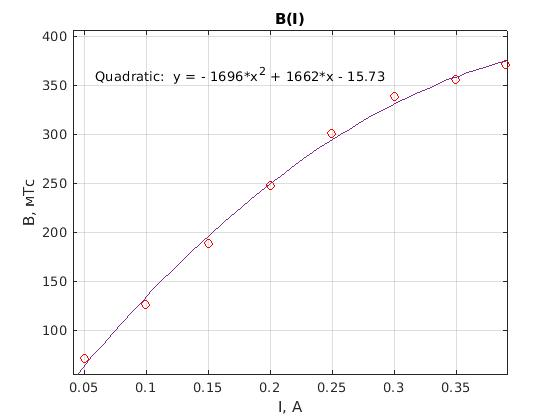
\includegraphics[width = 10 cm]{B(I).jpg}
    \caption{Измерение магнитных моментов шариков}
    \label{msh1}
\end{figure}
\end{center}

Видно, что при небольних значениях тока зависимость почти линейная, однако при больших видны значительные отклонения от прямой (парабола).


\subsection{Исследование магнетосопротивления образцов}

Подключим диск Корбино к электрической цепи. При помощи реостата $R_{2}$ установим ток через образец $I_{0} \simeq 25$ мА. Падение напряжения в случае расположения шириной вдоль поля -- $U_0 = (2,710\pm 0,002)$ В, шириной поперёк поля -- $U_0 = (2,853 \pm 0,002)$ В.

Вставим держатель с диском в зазор электромагнита. Снимим зависимость напряжения $U$ на образце от тока $I_{M}$ через обмотки магнита при фиксированном токе через образец $(I_{0} \simeq 25$ мА $) .$

\begin{table}[!h]
\begin{center}
\begin{tabular}{|c|c|}
\hline $U$, мВ & $I$, А\\
\hline 0,899 & 0,05 \\
\hline 1,213 & 0,10 \\
\hline 1,694 & 0,15 \\
\hline 2,175 & 0,20 \\
\hline 2,687 & 0,25 \\
\hline 3,143 & 0,30 \\
\hline 3,415 & 0,35 \\
\hline 3,552 & 0,39 \\
\hline
\end{tabular}
\end{center}
\caption{зависимость напряжения на образце от тока (диск)}
\end{table}

\begin{table}[!h]
\begin{center}
\begin{tabular}{|c|c|}
\hline $U$, мВ & $I$, А\\
\hline 0,898 & 0,05 \\
\hline 1,212 & 0,10 \\
\hline 1,696 & 0,15 \\
\hline 2,174 & 0,20 \\
\hline 2,687 & 0,25 \\
\hline 3,143 & 0,30 \\
\hline 3,414 & 0,35 \\
\hline 3,551 & 0,39 \\
\hline
\end{tabular}
\end{center}
\caption{зависимость напряжения на образце от тока (перевернутый диск)}
\end{table}


По полученным данным видно, что результат измерения не зависит от направления магнитного поля. 



Теперь  вместо диска Корбино подключим к измерительной цепи образец, имеющий форму пластинки. Реостатом $R_{2}$ установим в образце ток 10 мА. Измерим падение напряжения на образце в отсутствие магнитного поля.


Снимим зависимость напряжения $U$ на образце от тока через магнит при постоянном токе $I=10$ мА через образец. При измерениях длинная сторона образца должна быть направлена поперёк поля, а средняя (ширина) в одной серии опытов располагается вдоль, а в другой - поперёк поля.

полученный данные: 

\begin{table}[!h]
\begin{center}
\begin{tabular}{|c|c|}
\hline	$U$, мВ  & $I$, А  \\
\hline 2,890 & 0,05 \\
\hline 3,008 & 0,10 \\
\hline 3,142 & 0,15 \\
\hline 3,253 & 0,20 \\
\hline 3,384 & 0,25 \\
\hline 3,449 & 0,30 \\
\hline 3,488 & 0,35 \\
\hline 3,512 & 0,40 \\
\hline
\end{tabular}
\end{center}
\caption{зависимость напряжения на образце от тока (пластинка, поперек)}
\end{table}

\begin{table}[!h]
\begin{center}
\begin{tabular}{|c|c|}
\hline	$U$, мВ  & $I$, А  \\
\hline 2,782 & 0,05 \\
\hline 2,857 & 0,10 \\
\hline 2,959 & 0,15 \\
\hline 3,052 & 0,20 \\
\hline 3,142 & 0,25 \\
\hline 3,206 & 0,30 \\
\hline 3,242 & 0,35 \\
\hline 3,270 & 0,40 \\
\hline
\end{tabular}
\end{center}
\caption{зависимость напряжения на образце от тока (пластинка, вдоль)}
\end{table}


Для обработки результатов понадобятся данные с размерами диска и характеристиками приборов:

$InSb$; $D = 18\text{ мм}$; $d = 3\text{ мм}$; $h = 1,8\text{ мм}$ .





\section{Обработка результатов}

Построим калибровочный график $B(I_M)$, чтобы в дальнейшем использовать эти данные для интерполяции.


График полученной зависимости (и её аппроксимация):

\newpage

\begin{center}
\begin{figure}[h]
    \centering
    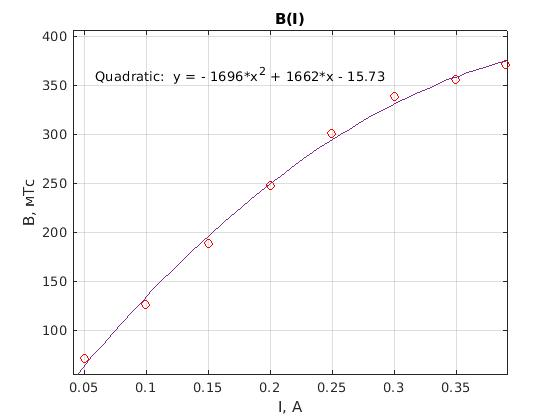
\includegraphics[width = 10 cm]{B(I).jpg}
    \caption{Измерение магнитных моментов шариков}
    \label{msh1}
\end{figure}
\end{center}

Видно, что при небольних значениях тока зависимость почти линейная, однако при больших видны значительные отклонения от прямой (парабола). 

Чтобы найти подвижность носителей необходимо посмотреть количественно на зависимость $R(B^2)$

\begin{table}[!h]
\begin{center}
\begin{tabular}{|c|c|c|c|}
\hline $\mathrm{B}^{2}$, $10^{-3} \text{ Тс}^2$ & $R_1$,\ мОм & $R_2$,\ мОм  & $R_3$,\ мОм  \\
\hline 5,1   & 35,96  & 289,0 & 278,2 \\
\hline 15,8  & 48,52  & 300,8 & 285,7 \\
\hline 35,4  & 67,76  & 314,2 & 295,9 \\
\hline 61,0  & 87,00  & 325,3 & 305,2 \\
\hline 90,6  & 107,48 & 338,4 & 314,2 \\
\hline 114,2 & 125,72 & 344,9 & 320,6 \\
\hline 126,7 & 136,60 & 348,8 & 324,2 \\
\hline 137,6 & 142,08 & 351,2 & 327,0 \\
\hline
\end{tabular}
\end{center}
\end{table}

Графики для 3-х серий $R(B^2)$, где 1-ая серия -- диск, 2-ая -- пластинка (поперек), 3-ая -- пластинка (вдоль):


\begin{center}
\begin{figure}[!h]
    \centering
    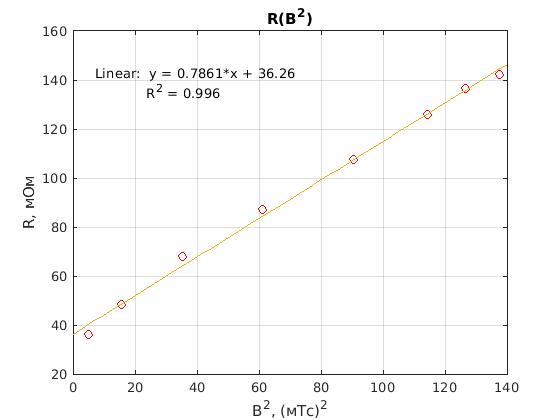
\includegraphics[width = 10 cm]{graph1(disk).jpg}
    \caption{график зависимсоти $R(B^2)$ для диска}
    \label{ser1}
\end{figure}
\end{center}

\begin{center}
\begin{figure}[!h]
    \centering
    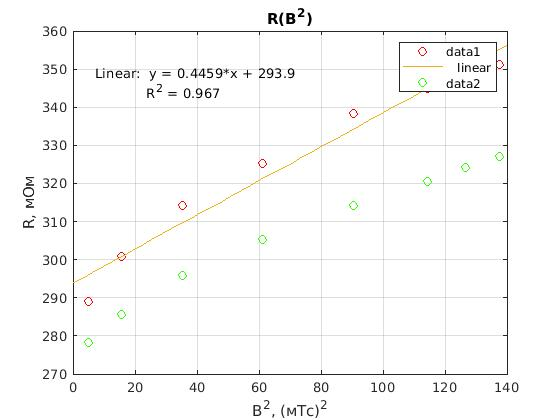
\includegraphics[width = 10 cm]{graph2(no_disk_poperek).jpg}
    \caption{график зависимсоти $R(B^2)$ для пластинка (поперек)}
    \label{ser2}
\end{figure}
\end{center}


\begin{center}
\begin{figure}[!h]
    \centering
    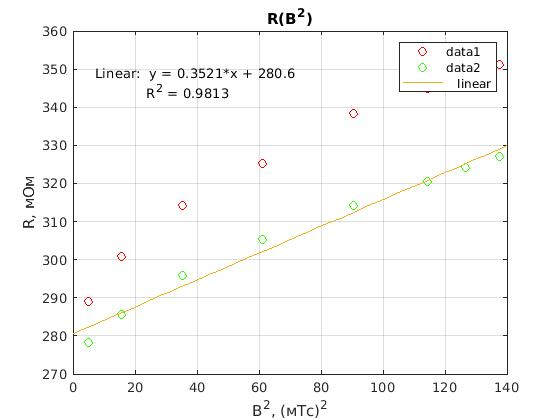
\includegraphics[width = 10 cm]{graph2(no_disk_vdol).jpg}
    \caption{график зависимсоти $R(B^2)$ для пластинка (вдоль)}
    \label{ser3}
\end{figure}
\end{center}

Тогда для каждой серии, по имеющимся $k,b$, где $y = kx + b$, можем рассчитать подвижность носителей:

\[ R = R_0\cdot\left[1 + (\mu B)^2\right]\]

\[ k \cdot A = b\mu^2 \Rightarrow \mu = \sqrt{\frac{k}{b} \cdot A} \]

где $A$ это коэффициент, зависящий от размерности осей $X,Y$, в данном случае он равен $10^{3}$.

Серия 1: $b_1 = 36,26\ \pm 4,18$, $k_1 = 0,78 \pm 0,05\ \Rightarrow \mu_1 = 4,64$ Тл$^{-1}$.

\[ \varepsilon_{\mu_1} = \frac{\sqrt{ (\frac{\partial \mu_1}{\partial k}) ^2 \cdot \sigma^2_{k} + (\frac{\partial \mu_1}{\partial b}) ^2 \cdot \sigma^2_{b}  }}{\mu_1} = \frac{\sqrt{  \frac{1}{4kb} \sigma^2_{k} + \frac{1}{4kb^3} \sigma^2_{b} }}{\sqrt{\frac{k}{b}}} = 0,08\]

Тогда $\mu_1 = 4,64 \pm 0,37$ Тл$^{-1}$.

%Серия 2: $b_2 = 293,90 \pm 8,84$, $k_2 = 0,45 \pm 0,10\ \Rightarrow \mu_2 = 1,24 \pm XX$.

%Серия 3: $b_3 = 280,60 \pm 4.10$, $k_3 = 0,35 \pm 0.05\ \Rightarrow \mu_3 = 1,12 \pm XX$.

Хоть для пластинок полученные данные и можно аппроксимировать как линейная зависимость $R(B^2)$, однако аппроксимация как квадратичной зависимости дает коэффициент корреляции на порядок ближе лежащий к 1, что говорит о том, что зависимость всё же не линейная (да и это наблюдяется исходи из характерного вида графика при больших $B^2$):

При этом теоретическая $\mu_{\text{теор}}$ = 7,7 Тл$^{-1}$. Значения не совпадают в пределах $2\sigma$, однако в порядок величины попали, но видимо не были учтены какие-то эффекты.

\newpage

\begin{center}
\begin{figure}[!h]
    \centering
    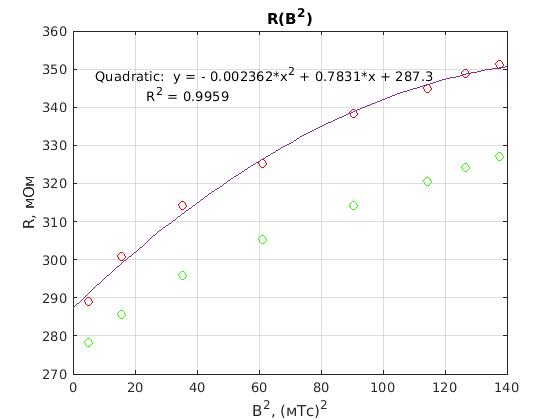
\includegraphics[width = 10 cm]{graph2(no_disk)(quadratic_1).jpg}
    \caption{график зависимсоти $R(B^2)$ для пластинка (поперек) (квадратичная аппроксимация)}
    \label{ser2_q}
\end{figure}
\end{center}

\begin{center}
\begin{figure}[!h]
    \centering
    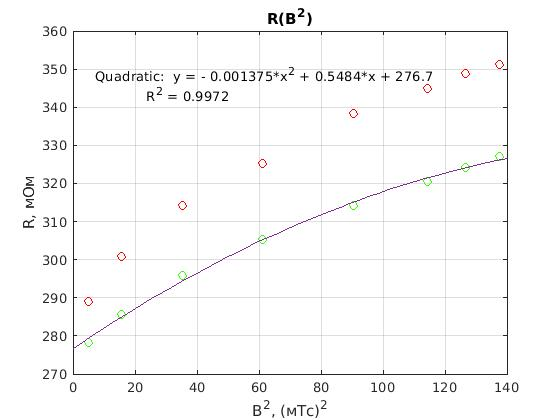
\includegraphics[width = 10 cm]{graph2(no_disk)(quadratic_2).jpg}
    \caption{график зависимсоти $R(B^2)$ для пластинка (вдоль) (квадратичная аппроксимация)}
    \label{ser3_q}
\end{figure}
\end{center}

Зная сопротивление диска в отсутствии магнитного поля и геометрические размеры образца, рассчитаем удельное споротивление материала образца $\sigma_0$ по формуле:

\[ \sigma_{0}=\frac{1}{2 \pi h R_{0}} \ln \frac{r_{2}}{r_{1}}= 437,92 \text{ (Ом} \cdot \text{см)}^{-1}\]

Рассчитаем концентрацию носителей тока:

\[ n=\frac{\sigma}{q \mu} = (5,89 \pm 0,24) \cdot 10^{18} \text{ м}^{-3} \]


Сравним полученные результаты со справочными:

\[ \sigma_{\text {тeop }}= 220 \left(\text{Ом} \cdot \text{см}\right)^{-1}\]

\[ n_{\text{тeop}}= 178 \cdot 10^{18} \text{ м}^{-3} \]

\section{Вывод}

Теоретическая зависимость выполняется для диска Корбина. А вот для пластинки тоже самое сказать нельзя, наблюдается нелинейное поведение кривой, для любого расположения, но при этом отличаются 
только наклоны кривых, сам характер кривых не изменяется. Полученные значения попадают в порядок с теоретическими, но при этом есть отклониния (более $3\sigma$), возможно связанные, как с неучтенными эффектами, так и с тем, что может быть другой материал (отличный от $InSb$).
\section{Литература}

\begin{enumerate}
\item \textbf{Лабораторный практикум по общей физике:} Учебное пособие. В трех томах. Т. 2. Электричество и магнетизм /Гладун А.Д., Александров Д.А., Берулёва Н.С. и др.; Под ред. А.Д. Гладуна - М.: МФТИ, 2007. - 280 с.

\end{enumerate}		
		


\end{document}